\documentclass[tikz, border=10pt]{standalone}
\usetikzlibrary{shapes}
\begin{document}
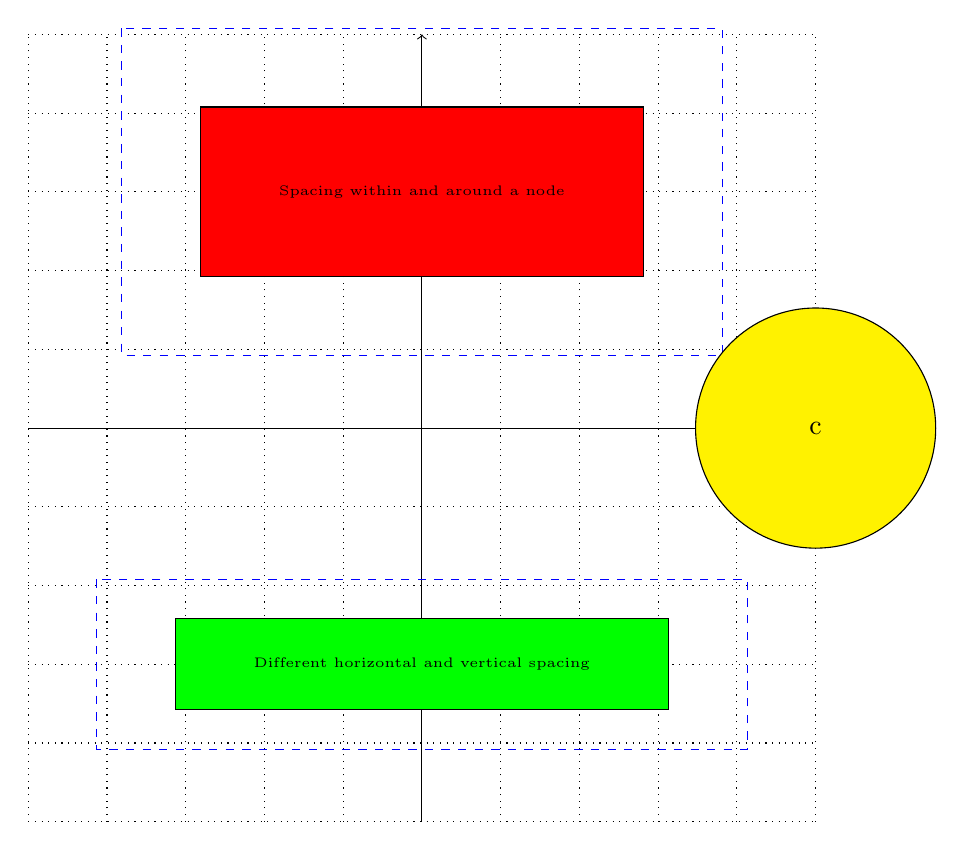
\begin{tikzpicture}
    \draw[thin, dotted] (-5, -5) grid[step=1] (5, 5);
    \draw[->] (-5, 0)--(5, 0);
    \draw[->] (0, -5)--(0, 5);
    \node[fill=red] (n) at(0, 3) [draw, rectangle, inner sep=1cm, outer sep=1cm]{\tiny Spacing within and around a node};
    \draw[dashed, blue] (n.north west)--(n.south west)--(n.south east)--(n.north east)--cycle;
    \node[fill=green] (n1) at(0, -3) [draw, rectangle, inner xsep=1cm, outer xsep=1cm, inner ysep=0.5cm, outer ysep=0.5cm]{\tiny Different horizontal and vertical spacing};
    \draw[dashed, blue] (n1.north west)--(n1.south west)--(n1.south east)--(n1.north east)--cycle;

    \node[fill=yellow] (c) at(5, 0) [draw, circle, inner sep=1cm, outer sep=1cm]{c};
    % \node 
\end{tikzpicture}
\end{document}